%\VignetteIndexEntry{xts: Extensible Time Series}
\documentclass{article}
\usepackage{hyperref}
\hypersetup{colorlinks,%
            citecolor=black,%
            linkcolor=blue,%
            urlcolor=blue,%
            }

\title{\bf xts: Extensible Time Series }
\author{Jeffrey A. Ryan \and Joshua M. Ulrich}
\date{May 18, 2008}

\usepackage{/Users/jryan/Desktop/R-2.7.0/share/texmf/Sweave}
\begin{document}

\maketitle
\tableofcontents

\section{Introduction}
The statistical language {\tt R}~\cite{R}
 offers the time-series analyst a variety of mechanisms
to both store and manage time-indexed data.  
Native {\tt R} classes potentially suitable
for time-series data include {\tt data.frame}, {\tt matrix}, {\tt vector}, and
{\tt ts} objects. Additional time-series tools have been subsequently introduced 
in contributed packages to
handle some of the domain-specific shortcomings of the native {\tt R} classes.
These include {\tt irts} from the {\tt tseries} package\cite{tseries},
{\tt timeSeries} from the {\tt Rmetrics} bundle\cite{rmetrics}, and
{\tt its}~\cite{its} and {\tt zoo}~\cite{zoo} from their 
respective packages. Each of these contributed classes provides unique solution
to many of the issues
related to working with time-series in R.

While it seems a bit paradoxical with all the current options
available, what {\tt R} really needed was one more
time-series class.  Why? Users of R have had many choices over the
years for managing time-series data. This variety has meant that
developers have had to pick and choose the classes they would support,
or impose the necessary conversions upon the end-user. With the sheer
magnitude of software packages available from CRAN, it has become a challenge
for users and developers 
to select a time-series class that will manage the needs of the
individual user, as well as remain compatible with the broadest audience.

What may be sufficient for one use --- say a quick correlation matrix may be
too limiting when more information needs to be incorporated 
in a complex calculation.
This is especially true for functions that rely on time-based indexes to
be manipulated or checked.

The previous solution to managing different data needs often
involved a series of {\tt as} calls,
to coerce objects from one type to another.  While this may
be sufficient for many cases, it is less flexible than allowing the users
to simply use the object they are accustomed to, or quite possibly require.
Additionally, all current coercion methods fail to maintain the original
object's data in its entirety.  Converting from a {\tt timeSeries} class to
{\tt zoo} would cause attributes such as 
{\em FinCenter}, {\em format}, and {\em recordIDs} to be lost.
Converting back to a {\tt timeSeries} would then add new
values different than the original.
For many calculations that do not modify the data, this is most likely
an acceptable side effect.  For functions that convert data ---
such as {\tt xts}'s {\tt to.period} --- it limits the value of the function,
as the returned object is missing
much of what may have been a factor in the original class consideration.

One of the most important additions the new {\tt xts} class makes
to the R user's
workflow doesn't use {\tt xts} at all, at least not explicitly.
By converting data to {\tt xts} inside a function, the function developer
is guaranteed to have to only manage a single class of objects. 
It becomes unecessary to write specific methods to handle different data.
While many functions do have
methods to accommodate different classes, most do not. Before {\tt xts}, the
{\tt chartSeries} function in the {\tt quantmod} package\cite{quantmod}
was only able to handle {\tt zoo} objects well.
Work had been done to allow for {\tt timeSeries} objects to be used as well, but
many issues were still being worked out.
With {\tt xts} now used internally, it is
possible to use \emph{any} of R's time-series classes.
Simultaneously saving development time and
reducing the learning/using curve for the end user.  The function now
simply handles whatever time-series object it receives
exactly as the user expects --- without complaint.
More details, as well as examples of incorporating {\tt xts} into
functions will be covered later in this document.

While it may seem that {\tt xts} is primarily a tool
to help make existing R code
more user-friendly, the opportunity to add exciting
(to software people) new functionality
could not be passed up.  To this end, {\tt xts} 
offers the user the ability to add
custom attributes to any object --- during its construction
or at any time thereafter.  Additionally,
by requiring that the index attribute be derived from one of
R's existing time-based classes, {\tt xts} methods can
make assumptions, while subsetting by time or date, that allow for
much cleaner and accurate data manipulation.

The remainder of this introduction will
examine what an {\tt xts} object consists of and
its basic usage, explain how developing with {\tt xts} can save
package development time, and finally will demonstrate
how to extend the class - informally
and formally.

\pagebreak
\section{The structure of {\tt xts}}
To understand a bit more of \emph{what an xts object can do}, it may
be beneficial to know \emph{what an xts object is}. This section
is intended to provide a quick overview of the basics of the
class, as well as what features make it unique.

\subsection{It's a {\tt zoo} in here}
At the core of an {\tt xts} object is a {\tt zoo} object from the package of
the same name. Simplified, this class contains an array of values
comprising your data (often in matrix form) and an index
attribute to provide information about
the data's ordering. Most of the details surrounding zoo
objects apply equally to xts. As it would be redundent to simply retell
the excellent introductory zoo vignette, the reader is advised to
read, absorb, and re-read that documentation to best
understand the power of this class. The authors of the {\tt xts}
package recognize that
{\tt zoo}'s strength comes from its
simplicity of use, as well as its overall flexibility.  What motivated the
{\tt xts} extension was a desire to have even more flexibility, while 
imposing reasonable constraints to make this class into a true time-based one.

\subsection{{\tt xts} modifications}
Objects of class {\tt xts} differ from objects of class 
{\tt zoo} in three key ways: the use of formal time-based
classes for indexing,
internal xts properties, and perhaps most uniquely
--- user-added attributes.

\subsubsection*{True time-based indexes}
To allow for functions that make use of {\tt xts} objects
as a general time-series object - it was necessary to
impose a simple rule on the class.  The index of each
{\tt xts} object \emph{must} be of a known and supported
time or date class.  At present this includes any one of
the following - Date, POSIXct, chron, yearmon, yearqtr, or
timeDate.  The relative merits of each are left to
the judgement of the user, though the first three are expected
to be sufficient for most applications.

\subsubsection*{Internal attributes: .CLASS, .ROWNAMES, etc.}
In order for one major feature of the {\tt xts} class
to be possible - the conversion and re-conversion of classes
to and from {\tt xts} - certain elements must be preserved within
the converted object.  These are for internal use, and
as such require little further explanation in an introductory
document. Interested readers are invited to examine the source as
well as read the developer documentation.

\subsubsection*{xtsAttributes}
This is what makes the xts class an \emph{extensible}
time-series class. Arbitrary attributes may be assigned
and removed from the object without causing issues with the data's display or
otherwise.  Additionally this is where \emph{other}
class specific attributes (e.g. \emph{FinCenter} from {\tt timeSeries})
are stored during conversion
to an xts object so they may be restored with {\tt reclass}.

\pagebreak
\section{Using the {\tt xts} package}
Just what is required to start using {\tt xts}?  Nothing more
than a simple conversion of your current time-series data with
{\tt as.xts}, or the creation of a new object with the {\tt xts} constructor.

\subsection{Creating data objects: {\tt as.xts} and {\tt xts}}
There are two equally valid mechanisms to create an {\tt xts}
object - coerce a supported time-series class to {\tt xts} with
a call to {\tt as.xts} or create a new object from scratch
with {\tt xts}.

\subsubsection*{Converting your \emph{existing} time-series data: {\tt as.xts}}
If you are already comfortable using a particular
time-series class in {\tt R}, you can still access
the functionality of {\tt xts} by converting your
current objects.

Presently it is possible to convert all the major
time-series like classes in {\tt R} to {\tt xts}. This list
includes objects of class:
matrix, data.frame, ts, zoo, irts, its, and timeSeries.
The new object will maintain all the necessary information
needed to {\tt reclass} this object back to its
original class if that is desired. Most classes
after re-conversion will be identical to similar modifications
on the original object, even
after sub-setting or other changes while an {\tt xts} object.

\begin{Schunk}
\begin{Sinput}
> require(xts)
> data(sample_matrix)
> class(sample_matrix)
\end{Sinput}
\begin{Soutput}
[1] "matrix"
\end{Soutput}
\begin{Sinput}
> str(sample_matrix)
\end{Sinput}
\begin{Soutput}
 num [1:180, 1:4] 50.0 50.2 50.4 50.4 50.2 ...
 - attr(*, "dimnames")=List of 2
  ..$ : chr [1:180] "2007-01-02" "2007-01-03" "2007-01-04" "2007-01-05" ...
  ..$ : chr [1:4] "Open" "High" "Low" "Close"
\end{Soutput}
\begin{Sinput}
> matrix_xts <- as.xts(sample_matrix, dateFormat = "Date")
> str(matrix_xts)
\end{Sinput}
\begin{Soutput}
An 'xts' object from 2007-01-02 to 2007-06-30 containing:
  Data: num [1:180, 1:4] 50.0 50.2 50.4 50.4 50.2 ...
 - attr(*, "dimnames")=List of 2
  ..$ : chr [1:180] "2007-01-02" "2007-01-03" "2007-01-04" "2007-01-05" ...
  ..$ : chr [1:4] "Open" "High" "Low" "Close"
  Indexed by: Class 'Date'  num [1:180] 13515 13516 13517 13518 13519 ...
  Original class: 'matrix'  
  xts Attributes:  
 NULL
\end{Soutput}
\begin{Sinput}
> df_xts <- as.xts(as.data.frame(sample_matrix), important = "very important info!")
> str(df_xts)
\end{Sinput}
\begin{Soutput}
An 'xts' object from 2007-01-02 to 2007-06-30 containing:
  Data: num [1:180, 1:4] 50.0 50.2 50.4 50.4 50.2 ...
 - attr(*, "dimnames")=List of 2
  ..$ : chr [1:180] "2007-01-02" "2007-01-03" "2007-01-04" "2007-01-05" ...
  ..$ : chr [1:4] "Open" "High" "Low" "Close"
  Indexed by:  POSIXct[1:180], format: "2007-01-02" "2007-01-03" "2007-01-04" "2007-01-05" ...
  Original class: 'data.frame'  
  xts Attributes:  
List of 1
 $ important: chr "very important info!"
\end{Soutput}
\end{Schunk}

A few comments about the above. {\tt as.xts} takes different arguments, depending
on the original object to be converted.  Some classes do not contain enough
information to infer a time-date class. If that is the case, POSIXct is used by
default. This is the case with both matrix and data.frame objects. In the preceding
examples we first requested that the new date format be of type 'Date'.  The
second example was left to the default {\tt xts} method
with a custom attribute added.

\subsubsection*{Creating new data: the {\tt xts} constructor}
Data objects can also be constructed directly from raw data with
the {\tt  xts} constructor function, in essentially the same way
a {\tt  zoo} object is created with the exception that at present
there is no equivelant {\tt zooreg} class.

\begin{Schunk}
\begin{Sinput}
> xts(1:10, Sys.Date() + 1:10)
\end{Sinput}
\begin{Soutput}
2008-06-10 2008-06-11 2008-06-12 2008-06-13 2008-06-14 2008-06-15 2008-06-16 
         1          2          3          4          5          6          7 
2008-06-17 2008-06-18 2008-06-19 
         8          9         10 
\end{Soutput}
\end{Schunk}

\subsection{{\tt xts} methods}
There is a full complement of standard methods to make use of the features
present in {\tt xts} objects. The generic methods currently
extended to {\tt xts} include ``{\tt [}'',
{\tt cbind}, {\tt rbind}, {\tt c}, {\tt str}, {\tt Ops},
{\tt print}, {\tt na.omit}, {\tt time}, {\tt index},
{\tt plot} and {\tt coredata}. In addition, most methods that can accept
zoo or matrix objects will simply work as expected.

A quick tour of some of the methods leveraged by {\tt xts}
will be presented here, including subsetting via ``{\tt [}'',
indexing objects with {\tt indexClass} and {\tt convertIndex},
and a quick look at plotting {\tt xts} objects with the {\tt plot}
function.

\subsubsection*{Subsetting}
The most noticable difference in the behavior of \texttt{xts} objects
will be apparent in the use of the ``{\tt [}'' operator. Using
special notation, one can use date-like strings to extract
data based on the time-index.  Using increasing levels of time-detail,
it is possible to subset the object by year, week, days - or even seconds.

The {\em i} (row)
argument to the subset operator ``{\tt [}'', in addition to accepting numeric
values for indexing,
can also be a character string, a time-based object, or a vector of either.
The format must left-specified with respect to the standard ISO:8601 
time format --- {\em ``CCYY-MM-DD HH:MM:SS''}~\cite{ISO}.  This means that for one 
to extract a particular month, it is necesssary to fully specify the 
year as well. To identify a particular hour, say all observations
in the eighth hour on January 1, 2007, one would likewise need
to include the full year, month and day - e.g. ``2007-01-01 08''. 

It is also possible to explicitly request a range of times via
this index-based subsetting, using a double colon ``::''
or the ISO-recommended ``/'' as the range seperater.
The basic form is {\em ``from::to''} or {\em ``from/to''},
where both {\em from} and {\em to}
are optional.  If either side is missing, it is interpretted as
a request to retrieve data from the beginning, or through the end of the
data object.

Another benefit to this method is that exact starting and ending
times need not match the underlying data - the nearest available
observation will be returned that is within the requested time
period.

The following example shows how
to extract the entire month of March 2007 - without having to
manually identify the index positions or match the underlying
index type. The results have been abbreviated to save space.
\begin{Schunk}
\begin{Sinput}
> matrix_xts["2007-03"]
\end{Sinput}
\end{Schunk}
\begin{Schunk}
\begin{Soutput}
               Open     High      Low    Close
2007-03-01 50.81620 50.81620 50.56451 50.57075
2007-03-02 50.60980 50.72061 50.50808 50.61559
2007-03-03 50.73241 50.73241 50.40929 50.41033
2007-03-04 50.39273 50.40881 50.24922 50.32636
2007-03-05 50.26501 50.34050 50.26501 50.29567
\end{Soutput}
\begin{Soutput}
...
\end{Soutput}
\end{Schunk}

Now extract all the data from the beginning through
January 7, 2007.
\begin{Schunk}
\begin{Sinput}
> matrix_xts['::2007-01-07'] # or matrix_xts['/2007-01-07']
\end{Sinput}
\end{Schunk}
\begin{Schunk}
\begin{Soutput}
               Open     High      Low    Close
2007-01-02 50.03978 50.11778 49.95041 50.11778
2007-01-03 50.23050 50.42188 50.23050 50.39767
2007-01-04 50.42096 50.42096 50.26414 50.33236
2007-01-05 50.37347 50.37347 50.22103 50.33459
2007-01-06 50.24433 50.24433 50.11121 50.18112
2007-01-07 50.13211 50.21561 49.99185 49.99185
\end{Soutput}
\end{Schunk}
Additional xts tools providing subsetting are the
{\tt first} and {\tt last} functions.
In the spirit of head and tail from
the {\em utils} recommended package, they allow
for string based subsetting, without forcing
the user to conform to the specifics of the
time index, similar in usage to the {\em by}
arguments of {\tt aggregate.zoo} and {\tt seq.POSIXt}.

Here is the first 1 week of the data
\begin{Schunk}
\begin{Sinput}
> first(matrix_xts, "1 week")
\end{Sinput}
\end{Schunk}
\begin{Schunk}
\begin{Soutput}
               Open     High      Low    Close
2007-01-02 50.03978 50.11778 49.95041 50.11778
2007-01-03 50.23050 50.42188 50.23050 50.39767
2007-01-04 50.42096 50.42096 50.26414 50.33236
2007-01-05 50.37347 50.37347 50.22103 50.33459
2007-01-06 50.24433 50.24433 50.11121 50.18112
2007-01-07 50.13211 50.21561 49.99185 49.99185
\end{Soutput}
\end{Schunk}

...and here is the first 3 days of the
last week of the data.
\begin{Schunk}
\begin{Sinput}
> first(last(matrix_xts, "1 week"), "3 days")
\end{Sinput}
\begin{Soutput}
               Open     High      Low    Close
2007-06-25 47.20471 47.42772 47.13405 47.42772
2007-06-26 47.44300 47.61611 47.44300 47.61611
2007-06-27 47.62323 47.71673 47.60015 47.62769
\end{Soutput}
\end{Schunk}
\subsubsection*{Indexing}
While the subsetting ability of the above makes
exactly {\em which} time-based class you choose
for your index a bit less relevant, it is none-the-less
a factor that is beneficial to have control over.

To that end, {\tt xts} provides facilities for indexing
based on any of the current time-based classes. These
include {\tt Date}, {\tt POSIXct}, {\tt chron}, {\tt yearmon},
{\tt yearqtr}, and {\tt timeDate}.  The index itself may
be accessed via the zoo generics extended to xts --- {\tt index} and
the replacement function {\tt index<-}.

It is also possible to directly query and set the
index class of an {\tt xts} object by using the respective functions
{\tt indexClass} and {\tt indexClass<-}.
Temporary conversion, resulting in a new object with the requested
index class, can be accomplished via the {\tt convertIndex} function.

\begin{Schunk}
\begin{Sinput}
> indexClass(matrix_xts)
\end{Sinput}
\begin{Soutput}
[1] "Date"
\end{Soutput}
\begin{Sinput}
> indexClass(convertIndex(matrix_xts, "POSIXct"))
\end{Sinput}
\begin{Soutput}
[1] "POSIXt"  "POSIXct"
\end{Soutput}
\end{Schunk}
\pagebreak
\subsubsection*{Plotting}

%\setkeys{Gin}{width=0.8\textwidth}
The use of time-based indexes within {\tt xts} allows
for assumptions to be made regarding the x-axis
of plots. The {\tt plot} method
makes use of the {\tt xts} function {\tt axTicksByTime}, which
heuristically identifies suitable tickmark locations
for printing given a time-based object. 

When {\tt axTickByTime} is called with its
{\tt ticks.on} argument set to ``auto'', the result
is a vector of suitably chosen tickmark locations.
One can also specify the specific points to use
by passing a character string to the argument
indicating which time period to create tickmarks on.
\begin{Schunk}
\begin{Sinput}
> axTicksByTime(matrix_xts, ticks.on = "months")
\end{Sinput}
\begin{Soutput}
Jan 02\n2007 Feb 01\n2007 Mar 01\n2007 Apr 01\n2007 May 01\n2007 Jun 01\n2007 
           1           31           59           90          120          151 
Jun 30\n2007 
         180 
\end{Soutput}
\end{Schunk}
A simple example of the plotting functionality
offered by this labelling can be seen here:
\begin{center}
\begin{Schunk}
\begin{Sinput}
> plot(matrix_xts[, 1], major.ticks = "months", minor.ticks = FALSE, 
+     main = NULL, col = 3)
\end{Sinput}
\end{Schunk}
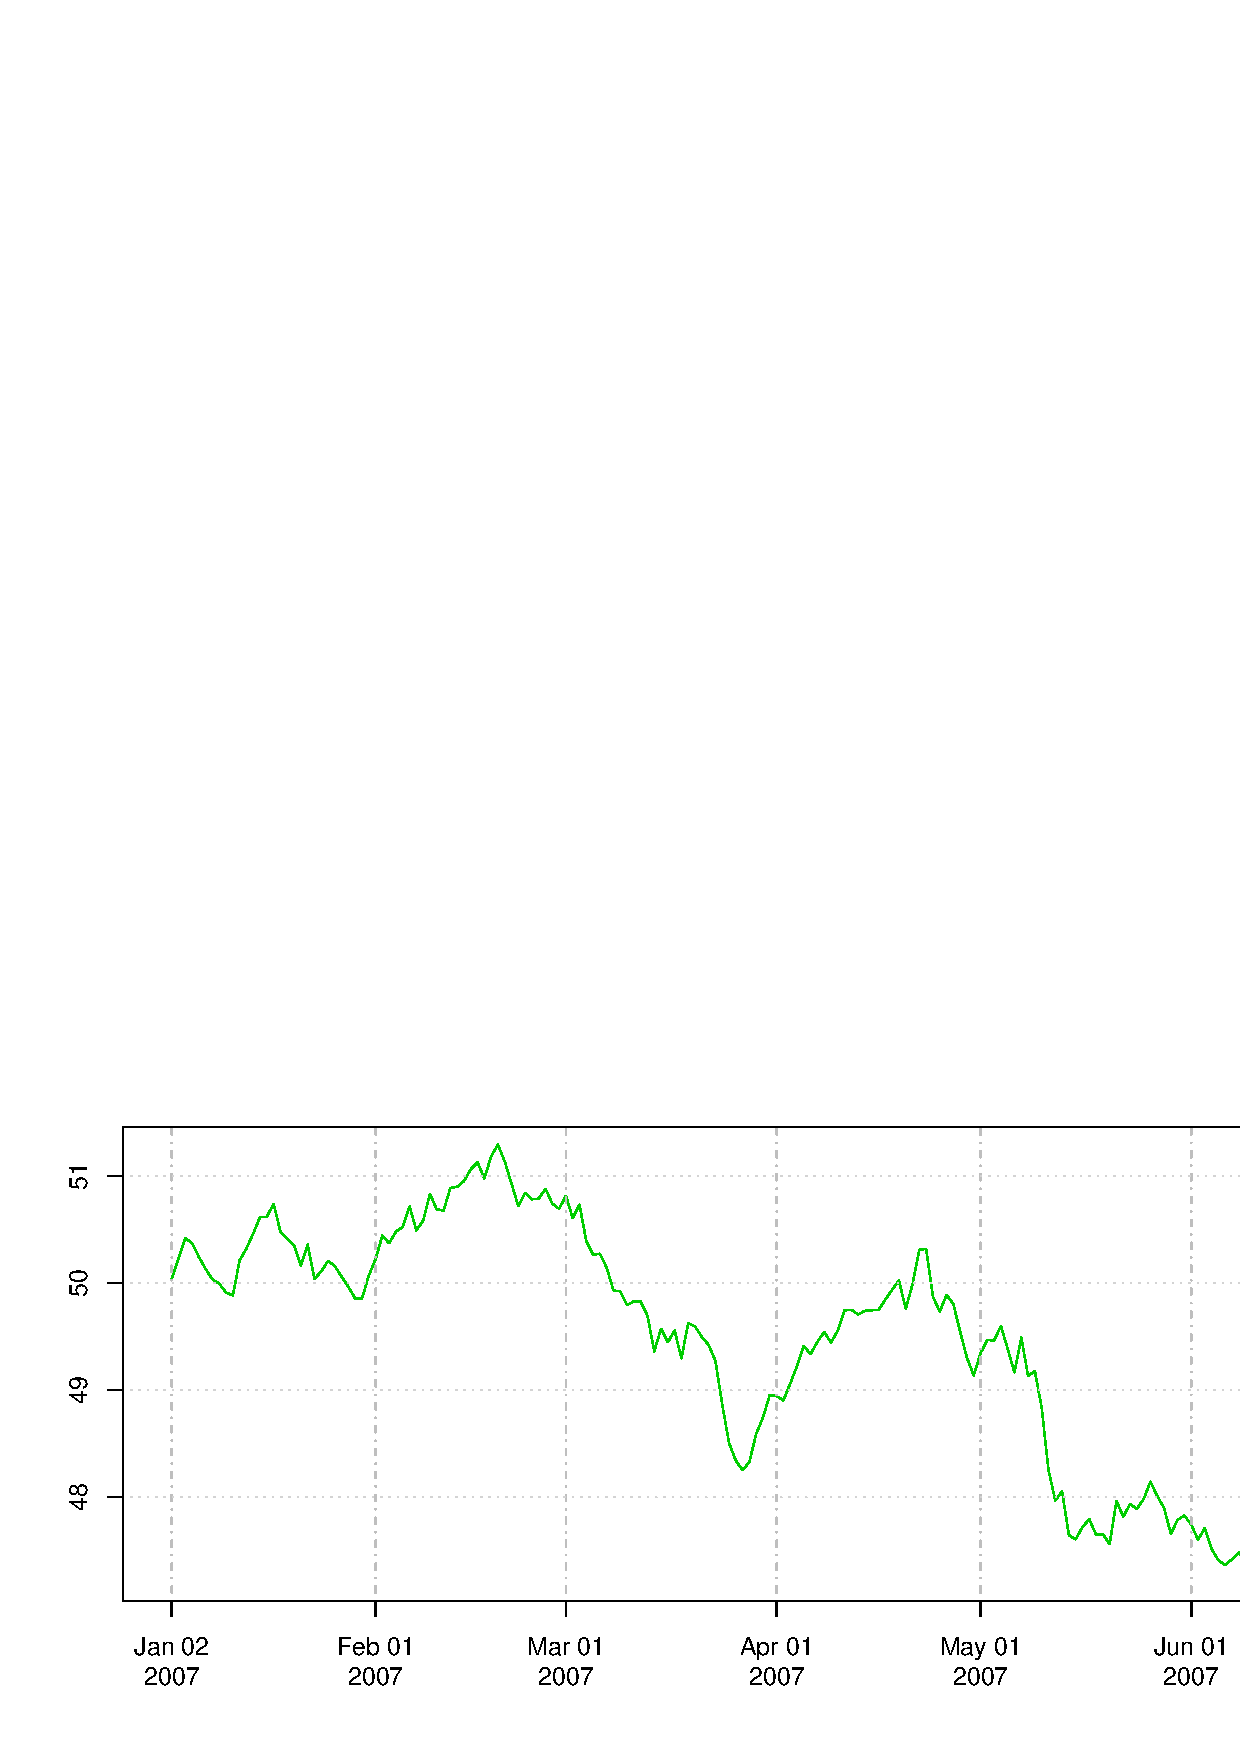
\includegraphics{xts-xtsplot}
\end{center}

\subsection{Restoring the original class - {\tt reclass} \& {\tt Reclass}}
By now you may be interested in some of the xts functionality
presented, and wondering how to incorporate it into
a current workflow --- but not yet ready to commit
to using it exclusively.

If it is desirable to only use the subsetting tools
for instance, a quick conversion to xts via {\tt as.xts}
will allow full access to the above subsetting tools. When
it is then necessary to continue your analysis using
the original class, it is as simple as calling the
function {\tt reclass} to return the object to its
original class.

\subsubsection*{(Re)converting classes manually: {\tt reclass}}
\begin{Schunk}
\begin{Sinput}
> # using xts-style subsetting doesn't work on non-xts objects
> sample_matrix['2007-06']
\end{Sinput}
\begin{Soutput}
[1] NA
\end{Soutput}
\begin{Sinput}
> # convert to xts to use time-based subsetting
> str(as.xts(sample_matrix)['2007-06'])
\end{Sinput}
\begin{Soutput}
An 'xts' object from 2007-06-01 to 2007-06-30 containing:
  Data: num [1:30, 1:4] 47.7 47.6 47.7 47.5 47.4 ...
 - attr(*, "dimnames")=List of 2
  ..$ : chr [1:30] "2007-06-01" "2007-06-02" "2007-06-03" "2007-06-04" ...
  ..$ : chr [1:4] "Open" "High" "Low" "Close"
  Indexed by:  POSIXct[1:30], format: "2007-06-01" "2007-06-02" "2007-06-03" "2007-06-04" ...
  Original class: 'matrix'  
  xts Attributes:  
 NULL
\end{Soutput}
\begin{Sinput}
> # reclass to get to original class back
> str(reclass(as.xts(sample_matrix)['2007-06']))
\end{Sinput}
\begin{Soutput}
 num [1:30, 1:4] 47.7 47.6 47.7 47.5 47.4 ...
 - attr(*, "dimnames")=List of 2
  ..$ : chr [1:30] "2007-06-01" "2007-06-02" "2007-06-03" "2007-06-04" ...
  ..$ : chr [1:4] "Open" "High" "Low" "Close"
\end{Soutput}
\end{Schunk}

This differs dramatically from the standard {\tt as.*****}
conversion though. Internally, key attributes of your
original data object are preserved and adjusted to
assure that the process introduces no changes other
than those requested.  Think of it as a smart {\tt as}.

Behind the scenes, {\tt reclass} has enormous value
in functions that convert all incoming data to {\tt xts}
for simplified processing. Often it is necessary to
return an object back to the user in the class he
is expecting --- following the principal of least surprise.
It is in these circumstances where {\tt reclass} can
turn hours of tedious development into mere minutes per function. More
details on the details of using this functionality
for developers will be covered in section \ref{developer},  
\textbf{Developing with xts}.

A user friendly interface of this \emph{reclass} functionality, though
implicit, is available in the {\tt Reclass} function.
It's purpose is to make it easy to preserve an object's attributes after calling
a function that is not programmed to be aware of your particular class.

\pagebreak
\subsubsection*{Letting xts handle the details: {\tt Reclass}}

If the function you require does not make use of
{\tt reclass} internally, it may still be possible to let
xts convert and reconvert your time-based object for you.
The caveat here is that the object returned:
\begin{quote}
\begin{itemize}
\item must be of the same length as the first argument to
the function.
\item intended to be coerced back to the class of the first
argument
\end{itemize}
\end{quote}
Simply wrapping the function
that meets these criteria in {\tt Reclass} will
result in an
attempt to coerce the returned output of the function

\begin{Schunk}
\begin{Sinput}
> z <- zoo(1:10,Sys.Date()+1:10)
> # filter converts to a ts object - and loses the zoo class
> (zf <- filter(z, 0.2))
\end{Sinput}
\begin{Soutput}
Time Series:
Start = 14041 
End = 14050 
Frequency = 1 
 [1] 0.2 0.4 0.6 0.8 1.0 1.2 1.4 1.6 1.8 2.0
\end{Soutput}
\begin{Sinput}
> class(zf)
\end{Sinput}
\begin{Soutput}
[1] "ts"
\end{Soutput}
\begin{Sinput}
> # using Reclass, the zoo class is preserved
> (zf <- Reclass(filter(z, 0.2)))
\end{Sinput}
\begin{Soutput}
2008-06-11 2008-06-12 2008-06-13 2008-06-14 2008-06-15 2008-06-16 2008-06-17 
       0.2        0.4        0.6        0.8        1.0        1.2        1.4 
2008-06-18 2008-06-19 2008-06-20 
       1.6        1.8        2.0 
\end{Soutput}
\begin{Sinput}
> class(zf)
\end{Sinput}
\begin{Soutput}
[1] "zoo"
\end{Soutput}
\end{Schunk}

The {\tt Reclass} function is still a bit experimental, and will
certainly improve in time, but for now provides at least
an alternative option to maintain your object's class
and attributes when the function you require can't on its own.

\subsection{Additional time-based tools}
In addition to the core {\tt xts} tools covered
above, there are more functions that are included
in xts to make the process of dealing with
time-series data easier. Some of these have been
moved from the package {\tt quantmod} to {\tt xts}
to make it easier to use them within other applications.

\subsubsection*{Calculate periodicity}
The {\tt periodicity} function provides
a quick summary as to the underlying
periodicity of most time-series like
objects. Primarily a wrapper to {\tt difftime}
it provides a quick and concise summary
of your data.
\begin{Schunk}
\begin{Sinput}
> periodicity(matrix_xts)
\end{Sinput}
\begin{Soutput}
Daily periodicity from 2007-01-02 to 2007-06-30 
\end{Soutput}
\end{Schunk}
\subsubsection*{Find endpoints by time}
Another common issue with time-series data
is identifying the endpoints with respect to
time. Often it is necessary to break data
into hourly or monthly intervals to calculate
some statistic. A simple call to {\tt endpoints}
offers a quick vector of values suitable
for subsetting a dataset by. Note that the first
element it zero, which is used to delineate the \emph{end}.
\begin{Schunk}
\begin{Sinput}
> endpoints(matrix_xts, on = "months")
\end{Sinput}
\begin{Soutput}
[1]   0  30  58  89 119 150 180
\end{Soutput}
\begin{Sinput}
> endpoints(matrix_xts, on = "weeks")
\end{Sinput}
\begin{Soutput}
 [1]   0   6  13  20  27  34  41  48  55  62  69  76  83  90  97 104 111 118 125
[20] 132 139 146 153 160 167 174 180
\end{Soutput}
\end{Schunk}
\subsubsection*{Change periodicity}
One of the most ubiquitous type of data
in finance is OHLC data (Open-High-Low-Close). Often is is necessary
to change the periodicity of this data to something
coarser - e.g. take daily data and aggregate to weekly
or monthly.  With {\tt to.period} and related wrapper
functions it is a simple proposition.
\begin{Schunk}
\begin{Sinput}
> to.period(matrix_xts, "months")
\end{Sinput}
\begin{Soutput}
           matrix_xts.Open matrix_xts.High matrix_xts.Low matrix_xts.Close
2007-01-31        50.03978        50.77336       49.76308         50.22578
2007-02-28        50.22448        51.32342       50.19101         50.77091
2007-03-31        50.81620        50.81620       48.23648         48.97490
2007-04-30        48.94407        50.33781       48.80962         49.33974
2007-05-31        49.34572        49.69097       47.51796         47.73780
2007-06-30        47.74432        47.94127       47.09144         47.76719
\end{Soutput}
\begin{Sinput}
> periodicity(to.period(matrix_xts, "months"))
\end{Sinput}
\begin{Soutput}
Monthly periodicity from 2007-01-31 to 2007-06-30 
\end{Soutput}
\begin{Sinput}
> to.monthly(matrix_xts)
\end{Sinput}
\begin{Soutput}
         matrix_xts.Open matrix_xts.High matrix_xts.Low matrix_xts.Close
Jan 2007        50.03978        50.77336       49.76308         50.22578
Feb 2007        50.22448        51.32342       50.19101         50.77091
Mar 2007        50.81620        50.81620       48.23648         48.97490
Apr 2007        48.94407        50.33781       48.80962         49.33974
May 2007        49.34572        49.69097       47.51796         47.73780
Jun 2007        47.74432        47.94127       47.09144         47.76719
\end{Soutput}
\end{Schunk}
The {\tt to.monthly} wrapper automatically requests that the
returned object have an index/rownames using
the {\tt yearmon} class. With the {\tt indexAt}
argument it is possible to align most series
returned to the end of the period, the beginning of the period,
or the first or last observation of the period --- 
even converting to something like {\tt yearmon} is supported.  The online
documentation provides more details as to additional
arguments.

\subsubsection*{Periodically apply a function}
Often it is desirable to be able to calculate a
particular statistic, or evaluate a function, over
a set of non-overlapping time periods. With the
{\tt period.apply} family of functions
it is quite simple.

The following examples illustrate a
simple application of the {\tt max} function
to our example data.
\begin{Schunk}
\begin{Sinput}
> # the general function, internally calls sapply
> period.apply(matrix_xts[,4],INDEX=endpoints(matrix_xts),FUN=max)
\end{Sinput}
\begin{Soutput}
2007-01-31 2007-02-28 2007-03-31 2007-04-30 2007-05-31 2007-06-30 
  50.67835   51.17899   50.61559   50.32556   49.58677   47.76719 
\end{Soutput}
\end{Schunk}

\begin{Schunk}
\begin{Sinput}
> # same result as above, just a monthly interface
> apply.monthly(matrix_xts[,4],FUN=max)
\end{Sinput}
\begin{Soutput}
2007-01-31 2007-02-28 2007-03-31 2007-04-30 2007-05-31 2007-06-30 
  50.67835   51.17899   50.61559   50.32556   49.58677   47.76719 
\end{Soutput}
\end{Schunk}
 
\begin{Schunk}
\begin{Sinput}
> # using one of the optimized functions - about 4x faster
> period.max(matrix_xts[,4], endpoints(matrix_xts))
\end{Sinput}
\begin{Soutput}
2007-01-31 2007-02-28 2007-03-31 2007-04-30 2007-05-31 2007-06-30 
  50.67835   51.17899   50.61559   50.32556   49.58677   47.76719 
\end{Soutput}
\end{Schunk}

In addition to {\tt apply.monthly}, there are
wrappers to other common time frames including:
{\tt apply.daily}, {\tt apply.weekly}, {\tt apply.quarterly},
and {\tt apply.yearly}.  Current optimized functions
include {\tt period.max}, {\tt period.min}, {\tt period.sum},
and {\tt period.prod}.

\pagebreak
\section{Developing with {\tt xts}}
\label{developer}
While the tools available to the xts \emph{user} are quite
useful, possibly greater utility comes from using xts
internally as a \emph{developer}. Bypassing
traditional S3/S4 method dispatch and
custom if-else constructs to handle different time-based
classes, {\tt xts} not only makes it easy to
handle all supported classes in one consistent manner,
it also allows the whole process to be invisible
to the function user.

\subsection{One function for all classes: {\tt try.xts}}
With the proliferation of data classes in R, it can be
tedious, if not entirely impractical, to manage interfaces to all
classes.

Not only does trying to handle every possible class present
non-trivial design issues, the developer is also forced
to learn and understand the nuances of up to eight or
more classes. For each of these classes it is then
ncessary to write and manage
corresponding methods for each case.

At best, this reduces the time available
to devote to core function functionality --- at worst
is a prime opportunity to introduce errors that
inevitibly come from this massive increase in code.

The solution to this issue is to use one class
internally within your package, or more generally your
entire workflow.  This can
be accomplished in one of two ways: force your users
to adopt the convention you do, or allow for
multiple object classes by relying on internal
code to convert to one consistent type.

Using the second approach offers the most end-user
flexibility, as class conversions are no longer
required simply to make use of package functionality. The
user's own workflow need not be interrupted with unproductive and
potentially error-prone conversions and reconversions.

Using the functionality of {\tt try.xts} and {\tt reclass} offered
by the xts package allows the developer an opportunity
to cleanly, and reliably, manage data with the least amount
of code, and the least number of artificial end-user restrictions.

An example from the xts package illustrates just how simple
this can be.

\begin{Schunk}
\begin{Sinput}
> period.apply
\end{Sinput}
\begin{Soutput}
function (x, INDEX, FUN, ...) 
{
    x <- try.xts(x, error = FALSE)
    FUN <- match.fun(FUN)
    xx <- sapply(1:(length(INDEX) - 1), function(y) {
        FUN(x[(INDEX[y] + 1):INDEX[y + 1]], ...)
    })
    reclass(xx, x[INDEX])
}
<environment: namespace:xts>
\end{Soutput}
\end{Schunk}

Some explanation of the above code is needed. The
{\tt try.xts} function takes three arguments, the first
is the object that the developer is trying to
convert, the second \ldots is any additional arguments to
the {\tt as.xts} constructor that is called internally
(ignore this for the most part --- though it should
be noted that this is an R dots argument \ldots), and the third is
a what the result of an error should be.

Of the three, {\tt error} is probably the most useful
from a design standpoint.  Some functions may not
be able to deal with data that isn't time-based. Simple
numerical vectors might not contain enough information
to be of any use. The \emph{error} argument
lets the developer decide if the function should be
halted at this point, or continue onward.
If a logical value, the result is
handled by R's standard error mechanism during the try-catch
block of code internal to {\tt try.xts}. If error is
a character string, it is returned to the standard output
as the message.  This allows for diagnostic messages to
be fine tuned to your particular application.

The result of this call, if successful (or if {\tt error=FALSE})
is an object that may be of class {\tt xts}.  If
your function can handle either numeric data or time-based
input, you can branch code here for cases you expect.  If your
code has been written to be more general
at this point, you can simply continue with your calculations,
the originally converted object will contain
the information that will be required to reclass it at the end.

A note of importance here: if you are planning on
returning an object that is of the original class, it
is important to not modify the originally coverted object - in this
case that would be the {\tt x} result of the {\tt try.xts} call.
You will notice that the function's result is assigned to
{\tt xx} so as not to impact the original converted function. If
this is not possible, it is recommended to copy the object first
to preserve an untouched copy for use in the {\tt reclass} function.

Which leads to the second part of the process of developing with
xts.

\subsection{Returning the original class: {\tt reclass}}
The {\tt reclass} function takes the object you are
expecting to return to your user (the result of all your
calculations) and optionally an {\tt xts} object
that was the result of the original {\tt try.xts} call.

It is important to stress that the {\tt match.to} object
\emph{must be an untouched object} returned from the
{\tt try.xts} call.  The only exception here is
when the resultant data has changed dimension --- as is
the case in the {\tt period.apply} example. As reclass
will try and convert the first argument to the orginal
class of the second (the original class passed to the function),
it must have the same general row dimension of the original.

A final note on using {\tt reclass}.  If the {\tt match.to} argument
is left off, the conversion will only be attempted if the object
is of class {\tt xts} and has a {\tt CLASS} attribute that is
not {\tt NULL}, else the object is simply
returned. Essentially if the object meant to be
reconverted is already of in the form needed by
the individual reclass methods, generally nothing
more needs to be done by the developer.

In many cases your function does not need to return
an object that is expected to be used in the same context
as the original. This would be the case for functions
that summarize an object, or perform some statistical analysis.

For functions that do not need the {\tt reclass} functionality,
a simple use of {\tt try.xts} at the beginning of the function
is all that is needed to make use of this single-interface
tool within {\tt xts}.

Further examples can be found in the {\tt xts} functions
{\tt periodicity} and {\tt endpoints} (no use of reclass), and
{\tt to.period} (returns an object of the original's class).
The package {\tt quantmod} also utilizes the {\tt try.xts}
functionality in its {\tt chartSeries} function --- allowing
financial charts for all time-based classes.

Forthcoming developer documentation will examine the functions
highlighted above, as well go into more detail on exceptional
cases and requirements.

\pagebreak
\section{Customizing and Extending xts}
As \emph{extensible} is in the name of
the package, it is only logical that it can be extended.
The two obvious mechanisms to make {\tt xts}
match the individual needs of a diverse user
base is the introduction of custom
attributes, and the idea of subclassing the entire
{\tt xts} class.

\subsection{{\tt xtsAttributes}}
What makes an R attribute an {\tt xtsAttribute}?
Beyond the sematics, xtsAttributes are designed to
persist once attached to an object, as well as not get
in the way of other object functionality.
All xtsAttributes are indeed R attributes, though 
the same can not be said of the reverse --- all
R attributes are \emph{not} xtsAttributes!

Attaching arbitrary attributes to most (all?) classes
other than {\tt xts} will cause the attribute to be displayed
during most calls that print the object.  While this isn't
necessarily devestating, it is often time unsightly, and sometimes
even confusing to the end user (this may depend on the quality your users).

xts offers the developer and end-user the opportunity to attach attributes
with a few different mechanisms - and all will be suppressed
from normal view, unless specifically called upon.

What makes an xtsAttribute special is that it
is principally a mechanism to store and view meta-data, that is,
attributes that would be seen with a call to R's
{\tt attributes}.

\begin{Schunk}
\begin{Sinput}
> str(attributes(matrix_xts))
\end{Sinput}
\begin{Soutput}
List of 6
 $ dim      : int [1:2] 180 4
 $ dimnames :List of 2
  ..$ : chr [1:180] "2007-01-02" "2007-01-03" "2007-01-04" "2007-01-05" ...
  ..$ : chr [1:4] "Open" "High" "Low" "Close"
 $ index    :Class 'Date'  num [1:180] 13515 13516 13517 13518 13519 ...
 $ class    : chr [1:2] "xts" "zoo"
 $ .CLASS   : chr "matrix"
 $ .ROWNAMES: chr [1:180] "2007-01-02" "2007-01-03" "2007-01-04" "2007-01-05" ...
\end{Soutput}
\begin{Sinput}
> str(xtsAttributes(matrix_xts))
\end{Sinput}
\begin{Soutput}
 NULL
\end{Soutput}
\begin{Sinput}
> xtsAttributes(matrix_xts) <- list(myattr = "my meta comment")
> attr(matrix_xts, "another.item") <- "one more thing..."
> str(attributes(matrix_xts))
\end{Sinput}
\begin{Soutput}
List of 8
 $ dim         : int [1:2] 180 4
 $ dimnames    :List of 2
  ..$ : chr [1:180] "2007-01-02" "2007-01-03" "2007-01-04" "2007-01-05" ...
  ..$ : chr [1:4] "Open" "High" "Low" "Close"
 $ index       :Class 'Date'  num [1:180] 13515 13516 13517 13518 13519 ...
 $ class       : chr [1:2] "xts" "zoo"
 $ .CLASS      : chr "matrix"
 $ .ROWNAMES   : chr [1:180] "2007-01-02" "2007-01-03" "2007-01-04" "2007-01-05" ...
 $ myattr      : chr "my meta comment"
 $ another.item: chr "one more thing..."
\end{Soutput}
\begin{Sinput}
> str(xtsAttributes(matrix_xts))
\end{Sinput}
\begin{Soutput}
List of 2
 $ myattr      : chr "my meta comment"
 $ another.item: chr "one more thing..."
\end{Soutput}
\end{Schunk}

In general - the only attributes that should be
handled directly by the user (\emph{without} the assistance
of xts functions) are ones returned by {\tt xtsAttributes}.
The additional attributes seen in the {\tt attributes}
example are for internal R and xts use, and if you expect
unbroken code, should be left alone.

\subsection{Subclassing {\tt xts}}
Subclassing xts is as simple as extending any other
S3 class in R.  Simply include the full class of
the xts system in your new class.

\begin{Schunk}
\begin{Sinput}
> xtssubclass <- structure(matrix_xts, class = c("xts2", "xts", 
+     "zoo"))
> class(xtssubclass)
\end{Sinput}
\begin{Soutput}
[1] "xts2" "xts"  "zoo" 
\end{Soutput}
\end{Schunk}

This will allow the user to override methods of xts and zoo,
while still allowing for backward compatibility with
all the tools of xts and zoo, much the way {\tt xts} benefits from
extending {\tt zoo}.

\section{Conclusion}
The {\tt xts} package offers both R developers and R users
an extensive set of time-aware tools for use in
time-based applications.  By extending the {\tt zoo} class,
xts leverages an excellent infrastructure tool into
a true time-based class.  This simple requirement for
time-based indexing allows for code to
make assumptions about the object's purpose, and facilitates
a great number of useful utilities --- such as time-based
subsetting.

Additionally, by embedding knowledge of the currently
used time-based classes available in R, xts can offer
the developer and end-user a single interface mechanism
to make internal class decisions user-driven.  This
affords developers an opportunity to design applications
for there intended purposes, while freeing up time
previously used to manage the data structures.

Future development of xts will focus on integrating
xts into more external packages, as well as additional useful
additions to the time-based utilities currently available
within the package.  An effort to provide external disk and
memory based data access will also be examined for potential
inclusion or extension.

\begin{thebibliography}{99}
\bibitem{zoo} Achim Zeileis and Gabor Grothendieck (2005):
\emph{ zoo: S3 Infrastructure for Regular and Irregular Time Series.}
Journal of Statistical Software, 14(6), 1-27. URL http://www.jstatsoft.org/v14/i06/

\bibitem{tseries} Adrian Trapletti and Kurt Hornik (2007):
\emph{tseries: Time Series Analysis and Computational Finance.} R package version 0.10-11.

\bibitem{rmetrics} Diethelm Wuertz, many others and see the SOURCE file (2007):
\emph{Rmetrics: Rmetrics - Financial Engineering and Computational Finance.}
R package version 260.72. http://www.rmetrics.org

\bibitem{its} Portfolio \& Risk Advisory Group and Commerzbank Securities (2006):
\emph{its: Irregular Time Series.} R package version 1.1.5.

\bibitem{ISO} International Organization for Standardization (2004):
\emph{ISO 8601: Data elements and interchage formats ---
      Information interchange --- Representation of dates and time}
URL http://www.iso.org

\bibitem{R} R Development Core Team:
\emph{R: A Language and Environment for Statistical Computing},
R Foundation for Statistical Computing, Vienna, Austria.
ISBN 3-900051-07-0, URL http://www.R-project.org

\bibitem{quantmod} Jeffrey A. Ryan (2008):
\emph{quantmod: Quantitative Financial Modelling Framework.}
R package version 0.3-5. URL http://www.quantmod.com
URL http://r-forge.r-project.org/projects/quantmod

\end{thebibliography}
\end{document}
